% !TeX spellcheck = en_US
\documentclass[
        %oneside,         	 %%retire % do in\'icio desta linha para n\~ao imprimir frente e verso 
        english,			
%	french,				
%	spanish, 
        brazil			        %% Idioma principal 
        ,<...>]{abntbibufjf}

\usepackage{lmodern}						
\usepackage[T1]{fontenc}		
\usepackage[utf8]{inputenc}		%% Para converter automaticamente acentos como digitados normalmente no teclado. Mude utf8 para latin1 se precisar. 
\usepackage{lastpage}			
\usepackage{indentfirst}		
\usepackage{color}			
\usepackage{graphicx}			
\usepackage{microtype} 
\usepackage[portuguese,ruled,lined]{algorithm2e}
\hyphenation{Con-si-de-ra-mos}
\hyphenation{me-lhor}
\hyphenation{res-pos-ta}
\hyphenation{re-qui-si-tos}
\hyphenation{Visua-lization}
\hyphenation{Wise-Arterial-Tree}
\hyphenation{Graphic-Ob-je-ct-Factories}
\hyphenation{admi-tân-cia}
\hyphenation{vis-co-elas-ti-ci-da-de}
\hyphenation{con-si-de-ra-do}
\hyphenation{in-de-pen-den-te-men-te}
\hyphenation{fun-ci-o-na-men-to}
\hyphenation{su-ces-si-va-men-te}
\hyphenation{com-pu-ta-ci-o-nal}
\hyphenation{geo-mé-tri-cas}

%\usepackage[portuguese]{babel}  
\usepackage{listings}
\usepackage[alf,bibjustif]{abntex2cite}
\usepackage{amsmath}
\usepackage{breqn}

%% -----------------------------------------------------------------------------

%% Obs.: Alguns acentos foram omitidos.

\titulo{Simulação de Escoamento Pulsátil em Modelos de Árvores Arteriais} %% Colocar, dentro de chaves {}, o t\'itulo do trabalho. Retirar % do inicio da linha seguinte se tiver subtitulo
%\subtitulo{subt\'itulo}  %% Retirar % do in\'icio desta linha se tiver subt\'itulo 
\autor{Igor Pires dos Santos} %%Colocar, dentro de chaves {}, o nome completo do autor
\autorR{Pires dos Santos, Igor} %%Colocar o sobrenome do autor, separado por v\'rgula, antes do restante do nome do autor. Ex.: Santos, Maria dos
\local{Juiz de Fora} %%Governador Valadares
\data{2021} %%Colocar o ano da entrega. Por exemplo, 2019
\orientador[Orientador:]{Rafael Alves Bonfim de Queiroz} %%Se precisar, troque [Orientador:] por [Orientadora:]
\coorientador[Coorientador:]{Ruy Freitas Reis} %% Colocar ``%'' no in\'icio desta linha se n\~ao tiver coorientador. Se precisar, troque por [Cooorientadora:]. 
\orientadorTitulo{Titula\c{c}\~ao} %%Colocar, dentro de chaves {}, a titula\c{c}\~ao do(a) orientador(a). Por exemplo, Prof. Dr.
\coorientadorTitulo{Titula\c{c}\~ao} %%Colocar, dentro de chaves {}, a titula\c{c}\~ao do(a) cooorientador(a). 
\instituicao{Universidade Federal de Juiz de Fora}
\faculdade{Programa de Pós-Graduação em Modelagem Computacional} %%Colocar, dentro de chaves {}, o nome da faculdade ou do instituto.
%\programa{Modelagem Computacional} %%Colocar, dentro de chaves {}, o nome do curso. Por exemplo: Programa de P\'os\mbox{-Gra}dua\c{c}\~ao em Matem\'atica
\objeto{Disserta\c{c}\~ao (Mestrado)}  %%Tese (Doutorado)  %%%Trabalho de Conclus\~ao de Curso (gradua\c{c}\~ao)
\natureza{Disserta\c{c}\~ao  %%Tese 
apresentada ao \insereprograma ~da   %% %%%Trabalho de conclus\~ao de curso apresentado \'a \inserefaculdade da %%%%SUBSTITUIR \'a POR ao SE FOR INSTITUTO    
Universidade Federal de Juiz de Fora como requisito parcial \`a obten\c{c}\~ao do 
t\'itulo de Mestre em  %%Doutor em    %%%grau de bacharel em 
Modelagem Computacional. %%Trocar Matem\'atica por outro, se precisar.
%\'Area de concentra\c{c}\~ao: %%PREENCHER   %%%N\~ao usar esta linha se for trabalho de conclus\~ao de curso da gradua\c{c}\~ao
}

%% Abaixo, prencher com os dados da parte final da ficha catalografica
\finalcatalog{1. Árvores arteriais. 2. Escoamento pulsátil. 3. Hemodinâmica Computacional. I. Alves Bonfim de Queiroz, Rafael, orient. II. Dr..} %% Aqui fica 
% escrito a palavra ``T\'itulo'' mesmo, nao o do trabalho. Se tiver coorientador, os dados ficam depois dos dados 
%% do orientador (II. Sobrenome, Nome do coorientador, coorient.) e antes de ``II. T\'itulo'', o qual passa a ``III. T\'itulo''.


%%Use o comando abaixo (retirando % de %\sistautordata) apenas se for usar o sistema autor-data (n\~ao o num\'erico) para refer\^encias.
%\sistautordata   


\begin{document}

%% ELEMENTOS PR\'E-TEXTUAIS

%% Capa
\inserecapa

%% Folha de rosto
\inserefolhaderosto

%% Ficha catalogr\'afica. AO IMPRIMIR, DEIXAR NO VERSO DA FOLHA DE ROSTO.
\inserecatalog  


%% Folha de aprovacao
\begin{folhadeaprovacao}
\inicfolhaaprov
        
Aprovada em (dia) de (m\^es) de (ano) %%Preencher com a data 
   
\vfill
\begin{center} BANCA EXAMINADORA \end{center}
\assinatura{\insereorientadorTitulo~\insereorientador \ - Orientador \\ Universidade Federal de Juiz de Fora}  %%Orientadora
%\assinatura{Professor Dr. \inserecoorientador \ - Coorientador \\ Universidade Federal de Juiz de Fora}
\assinatura{Titula\c{c}\~ao Nome e sobrenome \\ Universidade ???}
\assinatura{Titula\c{c}\~ao Nome e sobrenome  \\ Universidade ??} 
%\assinatura{...} %%RETIRE O % E PREENCHA SE PRECISAR
%  \assinatura{...}
%  \assinatura{...}
\end{folhadeaprovacao}
\cleardoublepage 


%% Dedicatoria. OPCIONAL. Colocar ``%'' no in\'icio de cada das 3 linhas abaixo, caso n\~ao queira.
 \begin{dedicatoria} 
  Dedico este trabalho ... 
 \end{dedicatoria}

 
%% Agradecimentos. OPCIONAL. CASO SEJA BOLSISTA, INSERIR OS DEVIDOS AGRADECIMENTOS.
\begin{agradecimentos}
Agrade\c{c}o aos ... 
\end{agradecimentos}


%% Ep\'igrafe. OPCIONAL
\begin{epigrafe} 
	A construção de modelos de árvores arteriais é importante para a realização de estudos hemodinâmicos. Neste trabalho, apresentam-se: (i) um esquema analítico para o cálculo das características locais das ondas de fluxo e pressão em modelos de árvores arteriais 1D (ii) um ambiente computacional desenvolvido para a simulação e visualização dos resultados no tocante à construção de modelos e estudos hemodinâmicos. Os resultados obtidos neste trabalho estão condizentes com dados numéricos relatados na literatura.
\end{epigrafe}


%% RESUMOS

%% Resumo em Portugu\^es. OBRIGAT\'ORIO.
\begin{resumo}

A construção de modelos de árvores arteriais é importante para a realização de estudos hemodinâmicos. Neste trabalho, apresentam-se: (i) um esquema analítico para o cálculo das características locais das ondas de fluxo e pressão em modelos de árvores arteriais 1D, (ii) um ambiente computacional desenvolvido para a simulação e visualização dos resultados no tocante à construção de modelos e estudos hemodinâmicos. Os resultados obtidos neste trabalho estão condizentes com dados numéricos relatados na literatura. \\[18pt]
Palavras-chave: Árvores arteriais. Escoamento pulsátil. Hemodinâmica Computacional. %finalizadas por ponto e inicializadas por letra maiuscula.
\end{resumo}
 
 
%% Resumo em Ingl\^es
\begin{resumo}[ABSTRACT]
 \begin{otherlanguage*}{english}

The construction of arterial tree's models is crucial in hemodynamics studies. In this work, the following are presented: (i) an analytical scheme based on physisc and mathematic laws to calculate the local charactheristics of the pressure and flux wave in 1D arterial tree's models, (ii) a computational environment desenvolved to simulate and visualize the results of the model's construction and hemodynamic studies. The results produced in this work are consistent to real morphometric data and numeric data related in the literature. \\[18pt]
Keywords: Árvores arteriais. Pulsatile flow. Computational hemodynamics. %finalizadas por ponto e inicializadas por letra maiuscula.
 \end{otherlanguage*}
\end{resumo}

%% Seguindo o mesmo modelo acima, pode-se inserir resumos em outras l\'inguas. 


%% Lista de ilustra\c{c}\~oes. OPCIONAL. 
\pdfbookmark[0]{\listfigurename}{lof}  

%Caso as ilustra\c{c}~oes do trabalho sejam todas do mesmo tipo (por exemplo, todas do tipo organograma), coloque % no in\\'icio das duas linhas abaixo. 
\ilustvaria   %Use este comando somente caso as ilustra\c{c}\~oes n\~ao sejam todas do mesmo tipo. 
\listilustvaria  %Use este comando somente caso as ilustra\c{c}\~oes n\~ao sejam todas do mesmo tipo e caso queira inserir a lista delas. 

%\listoffigures*  %Use este comando quando todas as ilustra\c{c}\~oes s\~ao do mesmo tipo e caso queira inserir a lista delas. Veja dicas no final deste arquivo.

\cleardoublepage
%% Lista de tabelas. OPCIONAL. 
\pdfbookmark[0]{\listtablename}{lot}
\listoftables*    %Coloque ``%'' no in\'icio desta linha, caso n\~ao queira lista de tabelas.
\cleardoublepage


%% Lista de abreviaturas e siglas. OPCIONAL
\begin{siglas} %%ALTERAR OS EXEMPLOS ABAIXO, CONFORME A NECESSIDADE
  \item[ABNT] Associa\c{c}\~ao Brasileira de Normas T\'ecnicas
%  \item[Fil.] Filosofia
%  \item[IBGE] Instituto Brasileiro de Geografia e Estat\'istica
%  \item[INMETRO] Instituto Nacional de Metrologia, Normaliza\c{c}\~ao e Qualidade Industrial
\end{siglas}

%% Lista de s\'imbolos. OPCIONAL
\begin{simbolos} %%ALTERAR OS EXEMPLOS ABAIXO, CONFORME A NECESSIDADE$R_s$: Resistência hidrodinâmica do segmento s\\
\item [$\eta$] Viscosidade Sanguínea \\
\item [$s$] Comprimento do segmento s\\
\item [$\Delta p_s$] Queda de pressão ao longo do segmento s\\
\item [$Q_s$] Fluxo sanguíneo através do segmento s \\
\item [$p_{perf}$] Pressão de perfusão na posição proximal \\
\item [$p_{term}$] Pressão terminal na posição distal \\
\item [$\mathbf{x}_{prox}$] Posição proximal do segmento raiz \\
\item [$r_p$] Raio do segmento pai \\
\item [$r_{esq}$] Raio do segmento filho à esquerda \\
\item [$r_{dir}$] Raio do segmento filho à direita \\
\item [$ktot$] Número de segmentos existentes na árvore \\
\item [$T$] Função custo para o CCO \\
\item [$\mu_p$] Dimensionalidade de $T$ \\
\item [$\lambda$] Dimensionalidade de $T$ \\
\item [$p$] Pressão \\
\item [$q$] Fluxo
\item [$t$] Tempo \\
\item [$x$] Coordenada axial ao longo do tubo arterial \\
\item [$c$] Velocidade de onda \\
\item [$Y$] Admitância do segmento arterial \\
\item [$A$] Área da seção transversal do segmento arterial \\
\item [$\rho$] Densidade do fluido \\
\item [$w$] Frequência angular \\
\item [$f$] Frequência da onda \\
\item [$L$] Comprimento do tubo arterial \\
\item [$k$] Geração do segmento na árvore \\
\item [$j$] Posição do segmento arteria na geração da árvore \\
\item [$E$] Módulo de Young \\
\item [$h$] espessura da parede do segmento de tubo arterial \\
\item [$p_f$] Pressão na posição proximal do segmento arterial \\
\item [$p_b$] Pressão na posição distal do segmento arterial \\
\item [$R$] Coeficiente de Reflexão \\
\item [$Y_e$] Admitância efetiva do segmento arterial \\
\item [$\alpha$] Número de Womersley \\
\item [$\epsilon$] Fator viscoso do segmento arterial \\
\item [$\mu$] Viscosidade no segmento arterial \\
\item [$J_p$] Funçao de Bessel de índice $p$ \\
%  \item[$ \forall $] Para todo
%  \item[$ \in $] Pertence
 \end{simbolos}

 
%% Sum\'ario
\pdfbookmark[0]{\contentsname}{toc}
\tableofcontents*
\cleardoublepage

%% ----------------------------------------------------------

%% ELEMENTOS TEXTUAIS
\textual


\chapter{INTRODU\c{C}\~AO}  %%Nesta linha, dentro de { }, digita-se em CAIXA ALTA, como apresentado aqui

Os benefícios que a Matemática Aplicada e Computacional pode proporcionar à medicina vascular estão condicionados à superação de algumas barreras. A primeira barreira está associada à construção do modelo geométrico da rede vascular, principalmente, a caracterização da estrutura geométrica dos casos ao nível da circulação periférica (arteríolas e capilares). A segunda está atrelada à descrição matemática e simulação do escoamento sanguíneo pulsátil em modelos geométricos de rede vascular.


 Sobre a primeira barreira, a construção de modelos geométricos de árvores arteriais \textit{in silico} pode ser obtida empregando algoritmos baseados em leis fractais \cite{Dawant1986,VanBeek1989} e princípios de otimização~\cite{Karch1999,Queiroz2013,Schreiner1993}. Modelos fractais assumem que as leis de ramificação são derivadas a partir de medições e repetitivamente são aplicadas em direção aos segmentos de vasos de menor calibre. Esta classe de modelos é relativamente fácil de gerar e reproduz as distribuições estatísticas dos segmentos (raios, comprimentos e ângulos de bifurcação) conhecidas a partir de medições. Porém, tal classe tem dificuldade, ou mesmo impossibilidade, de produzir um arranjo espacial anatomicamente apropriado dos segmentos. Pois, estes modelos são baseados em relações matemáticas que não controlam a estrutura geométrica dos segmentos durante o crescimento das redes vasculares. 


Já em relação à simulação do escoamento sanguíneo pulsátil, destacam-se que estudos de simulação hemodinâmica sistêmica têm sido frequentemente baseados em modelos de árvores arteriais para obter uma melhor compreensão de todos os aspectos relacionados ao escoamento sanguíneo, desde a propagação de ondas e análise do pulso de pressão, passando pelo diagnóstico e inclusive com aplicações no planejamento cirúrgico. Como a representação do sistema cardiovascular através de um modelo puramente 3D que leve em conta a estrutura geométrica exata de todos os vasos não é, no momento, viável computacionalmente, vêm sendo empregados modelos dimensionalmente heterogêneos conhecidos como 0D (zero-dimensional)--1D (unidimensional)--3D (tridimensional) \cite{Blanco2008,Formaggia2001,Urquiza2006}. Modelos 3D \cite{Peskin1972,Taylor1998} são utilizados para estudar em detalhe a hemodinâmica local de distritos arteriais de interesse, e a geometria destes modelos são provenientes de dados anatômicos obtidos normalmente via reconstrução de imagens médicas de pacientes específicos. Modelos 1D \cite{Avolio,Formaggia2003,Stergiopulos1992} são adotados para representar as artérias de maior calibre e a estrutura geométrica destes modelos pode ser construída a partir de dados anatômicos. Tais modelos são capazes de capturar os efeitos de propagação de ondas~\cite{Anliker1971,Duan}, a interação das reflexões destas ondas e dar como resultado um pulso de pressão e vazão com significado fisiológico tanto em artérias centrais como periféricas. No entanto, um modelo 1D de toda a árvore arterial sistêmica não é possível devido à falta de dados anatômicos precisos das regiões periféricas. Portanto, a árvore tem que ser truncada em algum nível. Normalmente, este truncamento é feito empregando modelos 0D \cite{Mates1988,Stergiopulos1992} conhecidos por terminais Windkessel à jusante da posição distal do modelo 1D para representar o comportamento de distritos arteriais relacionados com o nível de arteríolas e capilares. 

No tocante à descrição do escoamento sanguíneo pulsátil em árvores arteriais, adotou-se neste trabalho o modelo 1D proposto por Duan e Zamir~\cite{Duan}. Eles propuseram um modelo relativamente simples para representação da pressão sanguínea e do fluxo em um modelo de árvore arterial. Dentro de cada segmento de vaso, o escoamento sanguíneo foi calculado baseado em uma aproximação de Womersley, incluindo a elasticidade da parede, bem como a densidade do sangue e a viscosidade.

Este trabalho está organizado como segue. ORGANIZAÇÃO.

A principal motivação para a construção automática de modelos de árvores arteriais é a inviabilidade de ter dados anatômicos suficientes que permitam caracterizar em detalhe a estrutura geométrica de redes vasculares periféricas~\cite{Queiroz2013}. A representação adequada destas redes é necessária para modelar adequadamente o efeito dos leitos periféricos na hemodinâmica do sistema arterial humano, assim como também para permitir explorar as condições hemodinâmicas locais que se encontram na circulação periférica. Pois, os terminais Windkessel, os quais são modelos a parâmetros condensados~\cite{Stergiopulos1992}, representam de forma simplificada toda esta rede periférica rica em detalhe e que tem influência na resposta dos modelos 1D e 3D. De fato, os terminais Windkessel negligenciam a estrutura e as propriedades espaciais da microcirculação. 

A incidência maior de picos na onda de pressão ao percorrer a aorta já foi documentada como evidência para os efeitos da reflexão em árvores vasculares \cite{Kouchoukos,Lighthill,McDonald}. Enquanto as áreas de reflexão não podem ser completamente conhecidas ou localizadas, é geralmente aceito que a forma da onda de pressão é modificada significativamente enquanto progride pela aorta, de uma forma que só pode ser explicada por reflexões de onda.  Um entendimento mais claro da relação entre modificações e fatores de modificação motiva a busca e desenvolvimento de modelos matemáticos que determinam a forma da onda que o pulso de pressão toma em cada ponto ao percorrer uma árvore arterial. Dentro deste contexto, estudou-se o modelo de Duan e Zamir ~\cite{Duan}.

A construção de modelos geométricos para representação adequada dos leitos periféricos é mandatória para adquirir entendimento da influência destes nas respostas hemodinâmicas de modelos 1D e 3D do sistema cardiovascular. No entanto, a possibilidade de construir um modelo geométrico detalhado do ponto de vista anatômico de uma rede vascular real a partir da reconstrução de imagens médicas de ressonância magnética é ainda limitada~\cite{Harel2010}.

O cálculo correto das características locais das ondas de pressão e fluxo a medida que elas progridem ao longo de uma estrutura de árvore e se tornam modificadas por reflexões de onda possibilita capturar o pico de pressão existente no escoamento sanguíneo. Por isto, torna-se interessante e importante o estudo de modelos matemáticos como aquele de Duan e Zamir~\cite{Duan} para compreender melhor a hemodinâmica do sistema cardiovascular.

Os objetivos pretendidos e alcançados neste trabalho foram:
\begin{itemize}
	\item estudar e implementar o modelo matemático de Duan e Zamir que descreve o escoamento sanguíneo 1D em árvores arteriais;
	\item simular o escoamento sanguíneo em modelos de árvores arteriais sob diferentes cenários visando:
	\begin{itemize}
		\item analisar o impacto da viscosidade sanguínea;
		\item analisar o impacto da viscoelasticidade da parede do vaso;
		\item investigar o efeito da combinação da viscosidade sanguínea e viscoelasticidade da parede do vaso;
	\end{itemize} 
	\item desenvolver um sistema computacional para a análise de escoamento pulsátil em árvores arteriais, com os seguintes recursos:
	\begin{itemize}
		\item funcionamento multiplataforma;
		\item armazenamento consistente de todo modelo geométrico e suas propriedades;
		\item possibilitar análise de múltiplas árvores arteriais e modelos subsequentes;
		\item visualizar em tempo real as modificações feitas no modelo;
	\end{itemize} 
\end{itemize}

Este trabalho tem caráter interdisciplinar envolvendo áreas de Matemática Aplicada,
Computação, Biologia, Física e Medicina, o que torna fundamental o conhecimento
básico de cada área.

Primeiramente, estudou-se o modelo matemático de Duan e Zamir \cite{Duan}. Este estudo motivou o desenvolvimento de uma nova ferramenta computacional chamada~\textbf{IGU} (\textbf{Iterador Gráfico Universal}) para descrever o escoamento sanguíneo pulsátil em árvores arteriais. Inicialmente para verificar a robustez da ferramenta, buscou-se realizar algumas simulações semelhantes aquelas de Duan e Zamir a título de comparação. Destaca-se que a ferramenta~\textbf{IGU} foi desenvolvida em C++ e  contou com a utilização das bibliotecas Qt/OpenGL para ajudar na elaboração da interface gráfica.

AUMENTAR.


%=========================================================%

\chapter{Escoamento sanguíneo pulsátil em árvores arteriais}\label{sec:escoamento}

Nesta seção apresenta-se em detalhe a derivação do modelo matemático de Duan e Zamir \cite{Duan}, para o escoamento sanguíneo pulsátil em árvores arteriais.

A propagação de ondas em um tubo é governada pela equações da onda para a pressão $p(x,t)$ e fluxo $q(x,t)$ como seguem:
\begin{eqnarray}
\frac{\partial q}{\partial t} &=& -cY \frac{\partial p}{\partial x},
\label{01_p}\\
\frac{\partial p}{\partial t} &=& -\frac{c}{Y} \frac{\partial q}{\partial x}, 
\label{02_q}
\end{eqnarray}
nos quais $t$ é o tempo, $x$ é a coordenada axial ao longo do tubo, $c$ é a velocidade de onda, $Y = \frac{A}{\rho c}$ é a admitância e $A$ é a área da seção transversal do tubo, e $\rho$ é a densidade do fluido. Estas equações são baseadas na linearização das equações de movimento do fluido \cite{Fung,Lighthill}. Para uma onda harmônica simples, as equações (\ref{01_p}) e (\ref{02_q}) resultam em:
\begin{eqnarray}
p &=& \bar{p}_0 \exp\left[i\omega\left(t - \frac{x}{c}\right)\right] + R  \bar{p}_0 \exp\left[i\omega\left(t - \frac{2L}{c} + \frac{x}{c}\right)\right],
\label{03_p}\\
q &=& Y\left\{\bar{p}_0 \exp\left[i\omega\left(t - \frac{x}{c}\right)\right] -  R  \bar{p}_0 \exp\left[i\omega\left(t - \frac{2L}{c} + \frac{x}{c}\right)\right]\right\},
\label{04_1}
\end{eqnarray}
Onde $\omega = 2 \pi f$ é a frequência angular, $f$ é frequência em Hertz, $L$ é o comprimento do tubo, $\bar{p}_0$ a amplitude da onda incidente, $R$ é o coeficiente de reflexão definido pela razão entre as ondas refletidas pelas ondas que chegam no local de reflexão \cite{Fung,Karreman} e $i$ é a unidade imaginária ($i^2 = -1$).

As equações \eqref{03_p} e \eqref{04_1} para pressão e fluxo são aplicadas em cada segmento de vaso do modelo de árvore arterial, tomando $x = 0$ para o nó proximal e $x = L$ para o nó distal do segmento. Um segmento de vaso é definido pelo intervalo vascular entre dois locais de ramificação \cite{Zamir3}. No sistema arterial, as bifurcações são os locais de ramificação mais comuns~\cite{Zamir1}.

Em \cite{Duan}, um segmento de vaso é identificado por $(k,j)$, onde o primeiro $k$ representa o nível da geração e $j$ representa a ordem do segmento naquela geração, como mostrado na Figura \ref{fig1:arterial-tree}. Desta forma, a pressão e o fluxo ao longo de um segmento  $(k,j)$ do modelo de árvore arterial são dados por:
\begin{eqnarray}
p(k,j) &=& \bar{p}(k,j) \exp\left[i\omega\left(t - \frac{x(k,j)}{c(k,j)}\right)\right] \nonumber \\
&+& R(k,j)  \bar{p}(k,j) \exp\left[i\omega\left(t - \frac{2L(k,j)}{c(k,j)} + \frac{x(k,j)}{c(k,j)}\right)\right],
\label{05_p}\\
q (k,j) &=& Y(k,j)\left\{\bar{p}(k,j) \exp\left[i\omega\left(t - \frac{x(k,j)}{c(k,j)}\right)\right]\right. \nonumber \\
&-& \left. R(k,j)  \bar{p}(k,j) \exp\left[i\omega\left(t - \frac{2L(k,j)}{c(k,j)} + \frac{x(k,j)}{c(k,j)}\right)\right]\right\},
\label{06_q}
\end{eqnarray}
nos quais $\bar{p}(k,j)$ é a amplitude combinada do grupo de ondas progressivas no segmento $(k,j)$ e $R(k,j)$ é o coeficiente de reflexão no final daquele segmento, como é chamado a razão das ondas progressivas pelas atrasadas avaliadas no nó distal $x(k,j) = L(k,j)$. O grupo de ondas progressivas viaja no sentido positivo de $x(k,j)$, estas são compostas de ondas progressivas vindo de vasos acima deste, bem como, ondas refletidas na junção à montante $x(k,j) = 0$. O grupo de ondas atrasadas viaja no sentido oposto e é composto por ondas vindas de vasos à jusante como ondas refletidas na junção à jusante $x(k,j) = L(k,j)$. Assim, as equações \eqref{05_p} e \eqref{06_q} descrevem, respectivamente, as ondas de pressão e de fluxo localmente em um segmento $(k,j)$ do modelo de árvore, e localmente na posição $x(k,j)$ dentro deste segmento de vaso. As duas variáveis desconhecidas são a amplitude da pressão  $\bar{p} (k,j)$ e o coeficiente de reflexão $R (k,j)$, que são calculados na Seção~\ref{sec:pressao-fluxo} conforme proposto por Duan e Zamir~\cite{Duan}.  

\begin{figure}[!htbp] 
	\begin{center}
		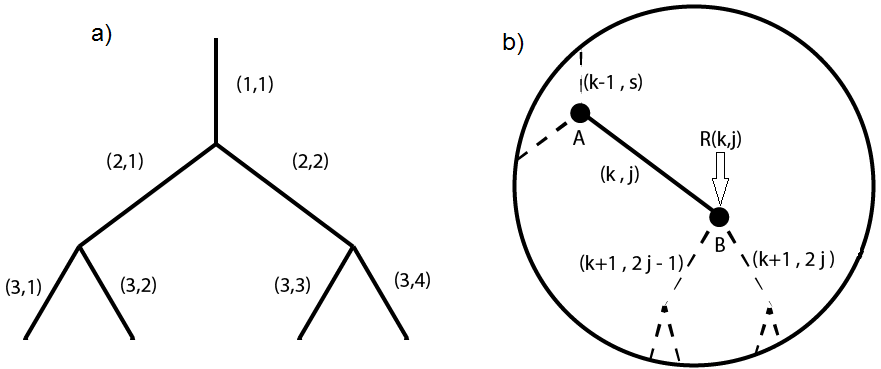
\includegraphics[scale = 0.5]{Figures/ArterialTree_Zamir.png}%
		\caption{Notação usada para identificar cada segmento de vaso $(k,j)$, onde $k$ é a geração/nível do vaso e $j$ é um número sequencial dentro daquela geração. }
		\label{fig1:arterial-tree}%
	\end{center}
\end{figure}

Os nós proximal e distal do segmento $(k,j)$ são denotados por $A$ e $B$, respectivamente. O coeficiente de reflexão $R(k,j)$ do segmento $(k,j)$ está associado ao nó distal $B$ (adaptada de \cite{Duan}).Na equação~\eqref{06_q}, tem-se a admitância característica para cada segmento dada por:
\begin{equation}
Y(k,j) = \frac{A(k,j)}{\rho(k,j)c(k,j)},
\label{eq:admitancia}
\end{equation}
nos quais $A(k,j)$ é a área da seção transversal do segmento $(k,j)$, $\rho(k,j)$ é a densidade do fluido dentro do vaso e $c(k,j)$ é a velocidade da onda correspondente. A admitância de um segmento é o inverso de sua impedância $Y = \frac{1}{Z}$, ou seja, é uma medida do quanto o segmento permite o fluxo.

Assumindo um segmento elástico de parede fina, a velocidade da onda $c(k,j)$ é calculada
por~\cite{Fung}:
\begin{equation}
c(k,j) = \sqrt{\frac{E(k,j) h(k,j)}{\rho(k,j) d(k,j)}},\label{eq:velocidade}
\end{equation}
onde $E(k,j)$ é o módulo de Young, $d(k,j)$ é o diâmetro do segmento $(k,j)$ e $h(k,j)$ é a espessura da parede do segmento, a qual neste estudo é dada por~\cite{Duan}: $h(k,j) = 0,05 d(k,j)$.

%-----------------------------------------------%
\section{Cálculo da pressão e do fluxo sanguíneo}\label{sec:pressao-fluxo}
Para determinar a pressão $\bar{p} (k,j)$ em um certo segmento $(k,j)$, aplica-se a condição de continuidade de pressão no nó proximal $A$ (ver Figura \ref{fig1:arterial-tree}). Escrevendo as componentes progressiva e atrasada da onda como $p_f (k,j)$ e $p_b (k,j)$ respectivamente, a pressão na posição proximal do segmento  $x(k,j) = 0$ é dada por:
\begin{equation}
\left[ p (k,j) \right]_A = \left[ p_f (k,j) \right]_A + \left[ p_b (k,j)\right]_A,
\label{09_p}
\end{equation}
nos quais as pressões $\left[ p_f(k,j) \right]_A$ e $\left[ p_b(k,j) \right]_A$ são expressas por:
\begin{eqnarray}
\left[ p_f(k,j) \right]_A &=& \bar{p}(k,j)\exp\left[ i\omega t\right],
\label{10_p_f}\\
\left[ p_b (k,j) \right]_A &=& R(k,j)\bar{p}(k,j)\exp\left[i\omega \left(t - \frac{2L(k,j)}{c(k,j)}\right) \right].
\label{11_p_b}
\end{eqnarray}

Similarmente, a pressão no segmento pai $(k-1,s)$ pode ser escrita como:
\begin{equation}
p(k-1,s) =  p_f(k-1,s) + p_b (k-1,s),
\label{12_p|_f}
\end{equation}
nos quais $s$ é um número sequencial do segmento pai e as pressões $ p_f (k-1,s)$ e $p_b (k-1,s)$ são dadas por:
\begin{eqnarray}
p_f (k-1,s) &=& \bar{p}(k-1,s)\exp\left[i\omega \left(t - \frac{x(k-1,s)}{c (k-1,s)}\right) \right],\\
\label{13_p_f}
p_b (k-1,s) &=& R (k-1,s)\bar{p}(k-1,s)\exp\left[ i\omega \left( t - \frac{2L(k-1,s)}{c(k-1,s)} + \frac{x(k-1,s)}{c(k-1,s)}\right) \right]. \nonumber
\end{eqnarray}

No nó distal do vaso superior, $x(k-1,s) = L(k-1,s)$, a pressão é dada por:
\begin{equation}
\left[ p(k-1,s) \right]_A = \left[ p_f(k-1,s)\right]_A + \left[ p_b(k-1,s) \right]_A,
\label{12_p|_f}
\end{equation}
nos quais 
\begin{eqnarray}
\left[ p_f(k-1,s) \right]_A &=& \bar{p}(k-1,s)\exp\left[ i\omega \left(t - \frac{L(k-1,s)}{c(k-1,s)}\right)\right],
\label{15_p_f}
\\
\left[ p_b(k-1,s) \right]_A &=& R(k-1,s)\bar{p}(k-1,s)\exp\left[i\omega \left( t - \frac{L(k-1,s)}{c(k-1,s)} \right) \right]. 
\label{16_p_b}
\end{eqnarray}

A condição de continuidade da pressão exige que na junção ela assuma um único valor, portanto
\begin{equation}
\left[ p_f(k-1,s) \right]_A + \left[ p_b (k-1,s) \right]_A = \left[ p_f(k,j) \right]_A + \left[ p_b(k,j) \right]_A.
\label{17_p_cont}
\end{equation}

Substituindo as equações \eqref{10_p_f}, \eqref{11_p_b}, \eqref{15_p_f} e \eqref{16_p_b} na equação \eqref{17_p_cont} e resolvendo para $\bar{p}(k,j)$, resulta em:
\begin{equation}
\bar{p} (k-1) =  \frac{\bar{p}(k-1,s)\left[1 + R(k-1,s)\right] \exp\left[ -\frac{i \omega L(k-1,s)}{c(k-1,s)}\right]}{1 + R(k,j)\exp{\left[ -2i\omega \frac{L(k,j)}{c(k,j)}\right]}}.
\label{18_barp}
\end{equation}

Conforme Duan e Zamir \cite{Duan}, para efeitos de cálculo da pressão e fluxo, adimensionalizam-se as pressões em \eqref{18_barp} em termos da pressão de entrada $p_0 = \bar{p}_0 \exp[i\omega t]$. Considerando $P(k,j) = \frac{p(k,j)}{p_0}$ e $\bar{P} (k,j) = \frac{\bar{p}(k,j)}{\bar{p}_0}$, a equação~\eqref{05_p} para o cálculo da pressão  pode ser expressa de forma adimensionalizada por:
\begin{equation}
P(k,j) = \bar{P}(k,j)\left\{\exp[ -i\beta(k,j) X(k,j)] + R(k,j) \exp[-i2\beta(k,j)] \exp[i\beta(k,j) X(k,j)]\right\}
\label{21_P},
\end{equation}
nos quais $\beta(k,j) = \frac{\omega(k,j) L(k,j)}{c(k,j)}$ e $X = \frac{x(k,j)}{L(k,j)}$. Similarmente, a equação\eqref{06_q} para o fluxo $q(k,j)$ pode ser obtida de forma adimensionalizada por:
\begin{equation}
Q(k,j) = M(k,j)\bar{P}(k,j)\left\{\exp\left[ -i\beta(k,j) X(k,j) \right]  - R(k,j) \exp[ -2i\beta(k,j)] \exp[i\beta(k,j) X(k,j)] \right\},
\label{23_Q}
\end{equation}
nos quais $Q(k,j) = \frac{q (k,j)}{q_0}$, $M = \frac{Y(k,j)}{Y(1,1)}$ e $q_0 = Y(1,1)p_0$. O cálculo da admitância $Y(1,1)$ na posição proximal do segmento raiz, ou seja, da artéria de alimentação é apresentado na próxima seção.

%------------------------------------------------------------%
\section{Cálculo dos coeficientes de reflexão e da admitância}

Para determinar os coeficientes de reflexão nas junções, consideram-se as duas junções $A$ e $B$ das extremidades de um segmento genérico $(k,j)$ de um modelo de árvore arterial conforme Duan e Zamir \cite{Duan}. Na posição distal $B$, o coeficiente de reflexão é definido por~\cite{Fung,Lighthill}:
\begin{equation}
R(k,j) = \frac{Y(k,j) - [Y_e(k+1,2j) + Y_e(k+1,2j-1)]}{Y(k,j) + [Y_e(k+1,2j) + Y_e(k+1,2j-1)]},
\label{27_R}
\end{equation}
nos quais $Y_e(k+1,2j-1)$ e $Y_e(k+1,2j)$ são admitâncias efetivas nos segmentos à jusante de $B$. Estas admitâncias são determinadas pela razão entre o fluxo e pressão naquela posição, que é dada por:
\begin{equation}
Y_e(k+1,s) = \frac{Y(k+1,s)\left\{1 - R(k+1,s)\exp{[-i2\beta(k+1,s)]}\right\}}{1 + R(k+1,s)\exp{[-i2\beta(k+1,s)]}},
\label{28_Ye}
\end{equation}
nos quais $s = 2j-1$ e $2j$ são os números sequenciais dos dois segmentos filhos e $R(k+1,s)$ é o coeficiente de reflexão na posição distal de cada segmento. Similarmente, $Y_e(k,j)$, a admitância na posição proximal $A$ do segmento $(k,j)$ pode ser dada por:
\begin{equation}
Y_e(k,j) = \frac{Y(k,j)\{1 - R(k,j)\exp{[-i2\beta(k,j)]}\} }{1 + R(k,j)\exp{[-i2\beta(k,j)]}}
\label{29_Ye}.
\end{equation}
Substituindo $R(k,j)$ da equação \eqref{27_R} em \eqref{29_Ye}, obtém-se  uma equação para cálculo das admitâncias efetivas ao longo do modelo de árvore arterial:
\begin{equation}
Y_e(k,j) = \frac{Y(k,j) [Y_e(k+1,2j) + Y_e(k+1,2j-1)+ i Y(k,j)\tan{\beta(k,j)}]}{Y(k,j) + i[Y_e(k+1,2j) + Y_e(k+1,2j-1)]\tan{\beta(k,j)}}.
\label{30_Ye}
\end{equation}

Em segmentos terminais, pode ser assumido que não ocorrem mais reflexões à jusante das posições distais destes segmentos, portanto a admitância efetiva destes segmentos é igual às suas admitâncias características. Adotando a equação \eqref{29_Ye}, todas as admitâncias efetivas podem ser determinadas percorrendo a árvore a partir dos segmentos terminais até o segmento raiz.

%--------------------------------------------------------------------------------%
\section{Cenários investigados com o modelo matemático do escoamento sanguíneo}
\label{sec:cenario}
A partir do modelo matemático aqui apresentado, os seguintes cenários são investigados nas simulações hemodinâmicas:
\begin{itemize}
	\item \textbf{cenário 1}: análise do impacto da viscosidade sanguínea ($\mu(k,j)$).\\
	Os efeitos da viscosidade sanguínea podem ser investigados por substituir a velocidade
	da onda $c(k,j)$ por uma velocidade da onda complexa~\cite{Duan1992}:
	\begin{equation} 
	c_v(k,j) = c(k,j) \sqrt{\epsilon},\label{eq:velocidade-complexa}
	\end{equation}
	onde $\epsilon$ é um fator viscoso que corresponde a um tubo elástico com restrições~\cite{Duan1992}. Seja $\alpha$ o
	número de Womersley adimensional
	\begin{equation}
	\alpha = r(k,j) \sqrt{\frac{\omega \rho(k,j)}{\mu(k,j)}},
	\end{equation}
	o fator viscoso $\epsilon$ é calculado por:
	\begin{equation}
	\epsilon = 1 - F_{10} (\alpha),
	\end{equation}
	onde a função $F_{10}$ é avaliada deste modo:
	\begin{equation}
	F_{10} (\alpha) = \frac{2 J_1(i^{1,5} \alpha)}{\alpha i^{1,5}J_0(i^{1,5} \alpha)},
	\end{equation}
	onde $J_p$ denota a função de Bessel de índice $p$.
	
	\item \textbf{cenário 2}: análise do impacto da viscoelasticidade da parede do vaso ($\phi_0$).\\
	A viscoelasticidade da parede do segmento é incorporado sustituindo o módulo de Young
	estático $E(k,j)$ por um módulo elástico complexo $E_c(k,j)$ no cálculo da velocidade $c(k,j)$ na equação~\eqref{eq:velocidade}
	da seguinte forma~\cite{Duan}:
	\begin{equation}
	E_c(k,j) = |E_c(k,j)| \exp\{i\phi\},\label{eq:Young}
	\end{equation}
	onde $\phi$ é o ângulo de fase entre a pressão e o deslocamento da parede do segmento \cite{Taylor3} expresso por $\phi = \phi_0 [1-\exp(-\omega)]$ e $|E_c (k,j)|$ corresponde ao módulo de Young fornecido para a simulação.
	
	\item \textbf{cenário 3}: efeitos da viscosidade sanguínea ($\mu(k,j)$) e da viscoelasticidade da parede do segmento ($\phi_0$) de forma combinada.
	
	Neste último cenário, utiliza-se a equação~\eqref{eq:Young} para determinar a velocidade da onda $c(k,j)$~\eqref{eq:velocidade} no modelo. Com este resultado, calcula-se  a equação~\eqref{eq:velocidade-complexa} para determinar a velocidade complexa $c_v(k,j)$ a ser considerada no modelo.
\end{itemize}
%--------------------------------------------------------------------------------%
\section{Algoritmo para o escoamento pulsátil}
\label{sec:algoritmo}

Para o cálculo correto da onda de pressão e fluxo presente nos modelos geométricos foi necessário determinar uma ordem de variáveis à se determinar:

\begin{itemize}
    \item Cálculo da admitância $(Y)$
    \item Cálculo da admitância efetiva $(Y_e)$
    \item Cálculo do coeficiente de reflexão $(R)$
    \item Cálculo da pressão média $(\bar{p})$
    \item Cálculo das ondas de pressão e fluxo $(P(x) e Q(x))$
\end{itemize}

As equações~\eqref{27_R} e~\eqref{28_Ye} expõem a necessidade de um valor $Y_e(k+1,2j)$ e $Y_e(k+1,2j-1)$ que fazem referência à valores de artérias adjacentes ao final deste segmento.
Entretanto, o caminho oposto é necessário para se resolver o valor da pressão média de cada segmento como visto na equação~\eqref{18_barp} que necessita da pessão efetiva do segmento superior $\bar{p}(k-1,s)$.
Com estes desafios em mente, a estrutura de dados desenvolvida utiliza de ponteiros para acessar os valores de artérias adjacentes. O algoritmo desenvolvido se dividiu em duas fases, em um primeiro momento realiza o cálculo dos segmentos finais ao segmento raiz (\textit{bottom-up}) e ,finalmente, da raiz aos segmentos finais (\textit{top-bottom}).


\begin{algorithm}[H]
	\SetAlgoLined
	\Entrada{\textit{\textbf{Modelo Arterial}},f(Hz),$\epsilon$,$\mu_0$,$\phi_0$ }
	\Inicio{
		Segmento a = raiz \textit{(começa a recursão pela raiz)}
		
		\Se{existe(a)}{
			Envia a recursão \textit{fase um}(a,f,$\mu_0$,$\phi_0$) e armazena $Y(k-1,s)$
		}
		\Se{existe($Y(k-1,s)$)}{
			Envia a recursão \textit{fase dois}(a,$p_0$,$Y(k-1,s)$)
		}
	}
\caption{Começo da recursão.}
\end{algorithm}

O valor complexo $(Y(k-1,s))$ armazenado é a admitância característica do segmento raiz, que é necessário para o cálculo da onda de fluxo como visto na equação~\eqref{23_Q}.

A linguagem escolhida permite que objetos sejam passados por ponteiros, portanto é possível passar toda a estrutura geométrica da árvore arterial através de um ponteiro para o segmento raiz. Cada segmento arterial que contêm as propriedades´:
\begin{table}[h]
\begin{tabular}{|c|c|c|c|}
	\hline
	Comprimento & $L$(cm) & Raio & $r$(cm) \\
	\hline
	Densidade & $\rho$(g/cm$^3$) & Viscosidade & $\mu$(cm$^2$/s) \\
	\hline
	Espessura da Parede & $h$ (cm) & Velocidade Ângular & $\omega$  \\
	\hline
	Velocidade de Onda & $c$(cm/s) & Alpha & $\alpha$ \\
	\hline
	Beta & $\beta$ & Módulo de Young & $E$(g/cms$^2$)\\
	\hline
	Admitância Característica & $Y$ & Admitância Efetiva & $Y_e$\\
	\hline
	Fator Viscoso & $\epsilon$ & Coeficiente de Reflexão & $R$ \\
	\hline
	Pressão Média & $\bar{p}$ & Pressão & $P(x)$\\
	\hline
	Fluxo & $Q(x)$ && \\
	\hline
\end{tabular}
\caption{Propriedades de cada segmento de vaso sanguíneo.}
\end{table}

Além destas informações o segmento possui ainda três ponteiros para segmentos adjacentes. Um destes para o segmento adjacente ao nó proximal, ou segmento de vaso superior $(k-1,s)$; Os restantes para os segmentos adjacentes ao nó distal, arbitrariamente segmento à esquerda e à direita, ou segmentos de vaso inferiores $(k+1,2j-1)$ e $(k+1,2j)$. Esta estrutura é equivalente à uma árvore duplamente encadeada, onde através de um único ponteiro para um segmento, é possível trafegar a árvore nos dois sentidos. Isto se torna particularmente útil quando é necessário acessar dados de outro segmento para o cálculo.

Os ponteiros permitem também determinar se a artéria é a raiz ou uma folha, caso o ponteiro para o segmento superior $(k-1,s)$ seja igual ao valor de Flag nulo se trata de um segmento raiz. Caso os dois segmentos $(k+1,2j-1)$ e $(k+1,2j)$ sejam iguais ao valor de Flag nulo se trata de uma folha.

A primeira fase do algoritmo foi desenvolvida para calcular os valores de admitância efetiva ($Y_e$) e coeficiente de reflexão ($R$) de cada segmento. Desta forma é necessário que a admitância efetiva dos segmentos inferiores ($Y_e(k+1,2j-1)$ e $Y_e(k+1,2j)$) já estejam definidos . Portanto, na primeira fase de cálculo é verificada a existência de segmentos inferiores e caso existam a recursão é enviada  até eles. Após o envio da recursão é feito o cálculo do segmento atual, desta forma o segmento inferior será definido antes do segmento atual.

\begin{algorithm}[H]
	\textbf{\textit{\textsl{\underline{fase um}}}}(a,f,$\epsilon$,$\mu_0$,$\phi_0$) \\
	\Entrada{Segmento $a$,f(Hz),$\epsilon$,$\mu_0$,$\phi_0$ }
	\Inicio{
		\Se{existe(a $\rightarrow$ esquerda)}{
			Envia a recursão \textit{fase um}(a $\rightarrow$ esquerda,f,$\mu_0$,$\phi_0$)
		}
		\Se{existe(a $\rightarrow$ direita)}{
			Envia a recursão \textit{fase um}(a $\rightarrow$ direita,f,$\mu_0$,$\phi_0$)
		}
		Calcula $c$,$\omega$,$\beta$ \\
		\Se{\textbf{não} viscoso}{
			Calcula $Y$
		}
		\Senao{
			Calcula $\alpha$,$\epsilon$,$E_v$,$c_v$e$Y_v$\\
			Adota $c = c_v$ e $Y = Y_v$
		}
		\Se{a $\in$ folha}{
			$Y_e = Y$ e $R = 0$
		}
		\Senao{
			Calcula $Y_e$ e $R$
		}
	}
	\caption{Primeira fase do cálculo, recursão \textit{(bottom-up)}.}
\end{algorithm}

No caso de seguimentos que possuam apenas um vaso inferior, a recursão é enviada para o segmento existente e o para o segmento ausente se assume que $Y_e = 0$.

A segunda fase do algoritmo foi desenvolvida para calcular o valor da pressão média e ondas de pressão e fluxo em cada segmento. Como visto na equação~\eqref{18_barp} o valor da pressão média requer o valor da pressão média do segmento superior $(k-1,s)$. Com isso, verifica-se se o segmento atual é a raiz, neste caso $\bar{p} = \bar{p_0}$, caso contrário é se faz necessário o cálculo de $\bar{p}$ com a equação~\eqref{18_barp}. Em seguida o valor das ondas de pressão e fluxo são adquiridos pelo domínio do segmento. Por último a recursão é enviada aos segmentos inferiores, desta forma se garante a existência de um valor $\bar{p}(k-1,s)$.

\begin{algorithm}[H]
\textbf{\textit{\textsl{\underline{fase dois}}}}(a,f,$\epsilon$,$\phi_0$) \\
\Inicio{
	\Se{a $\in$ raiz}{
		$\bar{p} = \bar{p_0}$
	}
	\Senao{
		Calcula $\bar{p}$
	}
	Calcula $P(X) e Q(X) \forall X \in [0,1])$ \\
	\Se{existe(a $\rightarrow$ adjacente)}{
		Envia a recursão \textit{fase dois}(a $\rightarrow$ esquerda,f,$\epsilon$,$\phi_0$)
	}
	\Se{existe(a $\rightarrow$ direita)}{
		Envia a recursão \textit{fase dois}(a $\rightarrow$ direita,f,$\epsilon$,$\phi_0$)
	}
}
\caption{Segunda fase do cálculo, recursão \textit{(bottom-up)}.}
\end{algorithm}

Ao término da execução os valores contidos na artéria são analisados separadamente. A onda de pressão e fluxo representa um conjunto de valores por segmento que precisam ser calculados e armazenados, para isto é preciso determinar a quantidade de pontos $N$ que serão analisados dentro do espaço $X \in [0,1]$, foi adotado $N = 101$. No caso da onda de pressão os valores encontrados para ramo de árvore deve resultar em um gráfico contínuo, isto é $P(k,j)(X=0) = P(k+1,2j)(X=q1)$ e $P(k,j)(X=0) = P(k+1,2j-1)(X=1)$.
	
%===================================================================================%
\chapter{Ferramenta computacional}\label{sec:modelagem}

Nesta seção apresentam-se detalhes da ferramenta computacional desenvolvida para simulação do escoamento sanguíneo em modelos de árvores arteriais. Com esta ferramenta, o usuário poderá  visualizar a estrutura da árvore arterial e depois da simulação hemodinâmica, visualizar curvas de distribuição de fluxo sanguíneo e pressão.

Esta ferramenta foi desenvolvida em C++ utilizando as bibliotecas comuns do Qt 5.15.0 \cite{QTClasses} e do OpenGL \cite{OpenGL}, que facilitam a criação da interface gráfica e a exibição de objetos, como árvores arteriais e gráficos. Ela foi nomeada de \textit{Iterador Gráfico Universal} (IGU), pois em sua modelagem de objetos qualquer objeto, que implemente a classe \textit{WiseObject} explicada na Seção~\ref{sec:objetos}, está apto para realizar iterações e desenhar-se através de diretivas OpenGL em um objeto de interface gráfica. Buscou-se no desenvolvimento desta ferramenta alto grau de generalização para que possa ser utilizada por diferentes objetos dentro do ambiente. Além de árvores arteriais menciona-se que a ferramenta itera diferentes estruturas de dados, entre eles grafos e autômatos, por isto uma nomenclatura genérica.

A Figura~\ref{fig1:gui} ilustra a ferramenta desenvolvida. À seguir, apresentam-se em detalhes a implementação computacional realizada.

\begin{figure}[!htbp]
	\centering
	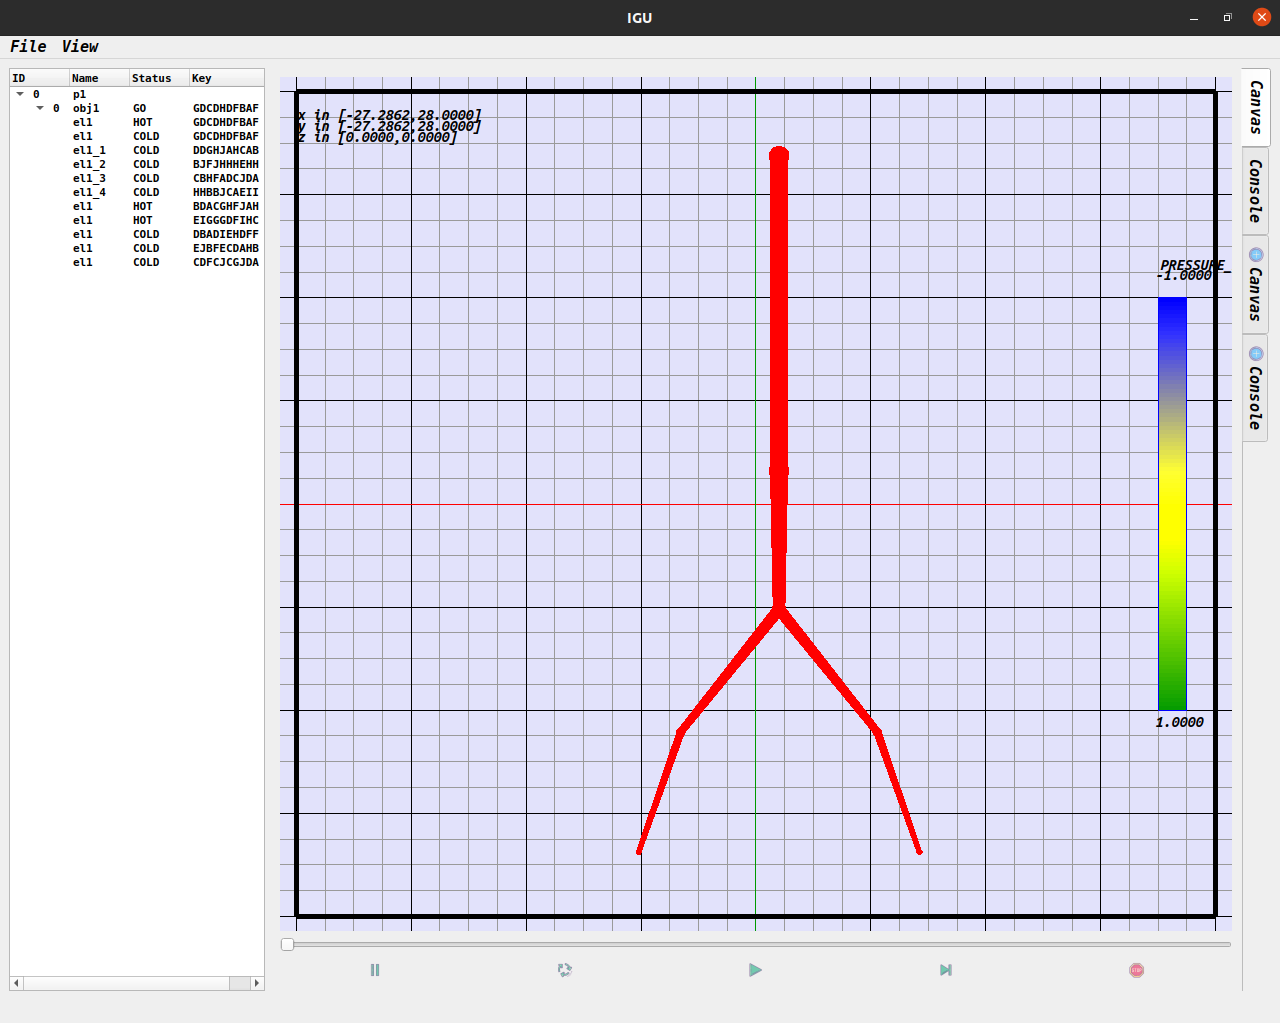
\includegraphics[scale=0.25]{Figures/IGU.png}
	\caption{Interface gráfica da ferramenta desenvolvida.}
	\label{fig1:gui}
\end{figure}

Através da modelagem de classes no paradigma do C++ \cite{AlanParker}, foi possível realizar diversas generalizações para ampliar a quantidade de objetos que podem ser inseridos neste modelo de classes. Na seção seguinte apresentamos um esquema de classes virtuais, ou abstratas, que foram criadas para facilitar o manuseio dos objetos dentro do ambiente computacional e prover funções básicas, a classe \textit{WiseElement}. Denomina-se um elemento inteligente aquele que herdar esta classe \textit{WiseElemet}.

%--------------------------------------------------------------------------------%
\section{Estrutura de Dados}\label{sec:estrutura}

Nesta seção apresentam-se detalhes da estrtura de dados adotada no funcionamento da ferramenta computacional. Como mencionado na Seção~\ref{sec:algoritmo} é utilizada uma estrutura de ponteiros que é capaz de armazenar todas as informações do modelo geométrico da árvore arterial. A ferramenta computacional foi desenvolvida para ser capaz de armazenar, carregar e iterar este modelo bem como gerar novas estruturas para visualização.

Baseando-se na estrutura básica presente nos arquivos de visualização do \textit{VTK}(\textit{Visualization ToolKit}) a estrutura presente na Figura~\ref{fig2:wiselement} foi criada.

\begin{figure}[!htbp]
	\centering
	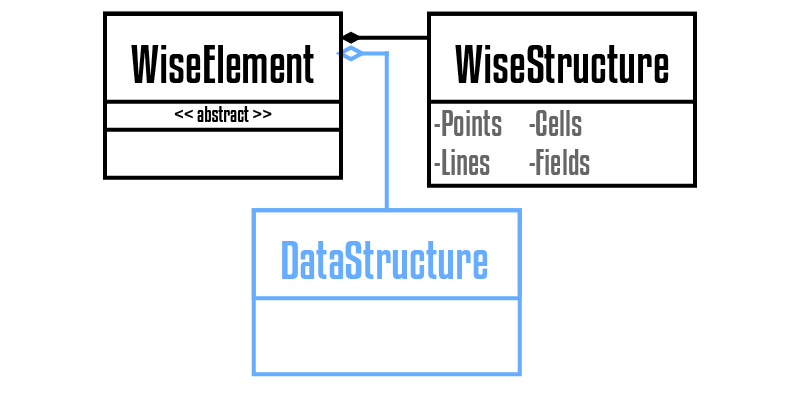
\includegraphics[scale=1]{Figures/WiseElement.png}
	\caption{Representação de classses de um elemento inteligente. WiseElement a classe abstrata base e seus componentes:WiseStructure representa a estrutura contida em um arquivo VTK e DataStructure representa a estrutura de ponteiros e variáveis utilizadas na iteração. Tingido de azul as estruturas que nem sempre estão presentes.}
	\label{fig2:wiselement}
\end{figure}

A Figura~\ref{fig2:wiselement} mostra que um elemento inteligente é composto por duas outras estruturas, uma delas utiliza pontos, linhas, células, linhas e campos para determinar estruturas geométricas. Isto foi feito para facilitar a leitura e escrita de objetos, pois a classe WiseElement foi desenvolvida para construir a estrutura abstrata à partir destas informações. A segunda estrutura não está sempre presente pois como veremos é custoso manter em memória esta estrutura para todos os elementos. Portanto, todos os elementos inteligente obedecem à máquina de status contida na Figura~\ref{fig3:wiselementstatus}.

\begin{figure}[!htbp]
	\centering
	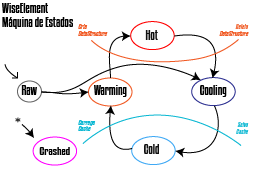
\includegraphics[scale=1]{Figures/WiseElementStatus.png}
	\caption{Máquina de Status que contola o funcionamento de um elemento inteligente.}
	\label{fig3:wiselementstatus}
\end{figure}

Todo elemento inteligente é criado no estado \textit{Raw}, ou cru, que representa um elemento ainda sem estruturas básicas carregadas. Uma vez que as estruturas são inseridas e verificadas o elemento muda para o status \textit{Warming} ou \textit{Cooling}, respectivamente esquentando ou esfriando, que estão representados na Figura~\ref{fig4:wiselementwarming}.

\begin{figure}[!htbp]
	\centering
	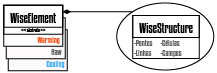
\includegraphics[scale=1]{Figures/WiseElementWarming.png}
	\caption{Elemento inteligente enquanto no estado \textit{Warming}.}
	\label{fig4:wiselementwarming}
\end{figure}


%=========================================================%

\begin{citacao}
As cita\c{c}\~oes diretas, no texto, com mais de tr\^es linhas, devem ser destacadas 
com recuo de 4 cm da margem esquerda, com letra menor que a do texto utilizado 
e sem as aspas. [...] Para enfatizar trechos da cita\c{c}\~ao, deve-se destac\'a-los indicando esta 
altera\c{c}\~ao com express\~ao grifo nosso entre par\^enteses, ap\'os a chamada da cita\c{c}\~ao, ou grifo 
do autor, caso o destaque j\'a fa\c{c}a parte da obra consultada. (ASSOCIA\c{C}\~AO BRASILEIRA DE NORMAS 
T\'ECNICAS, 2002, p. 2-3)
\end{citacao}

%As instru\c{c}\~oes aqui contidas buscam ajudar a direcionar e orientar quanto \`a padroniza\c{c}\~ao das monografias, dissertac\~oes e teses na UFJF. 
%Ser\~ao apresentados alguns exemplos de refer\^encias apenas como modelo de documento. Detalhes completos sobre como apresentar as refer\^encias se 
%encontram na norma ABNT NBR 6023:2018. Mais informa\c{c}\~oes sobre as normas de padroniza\c{c}\~ao s\~ao encontradas diretamente nas bibliotecas da UFJF e em 
%http://www.ufjf.br/biblioteca/servicos/normalizacao-2

%\chapter{NOME DO CAP\'ITULO} %%Nesta linha, dentro de { }, digita-se em CAIXA ALTA, como apresentado aqui

%Ap\'os a introdu\c{c}\~ao, segue-se o elemento desenvolvimento. Este elemento obrigat\'orio \'e que ir\'a desenvolver a ideia principal do trabalho. 
%\'E o elemento mais longo, podendo ser dividido em v\'arias se\c{c}\~oes %(prim\'arias, secund\'arias, etc.) 
%e subse\c{c}\~oes que devem conter texto. 

%Apresentamos nesta p\'agina um exemplo de nota \footnote{As notas devem ser digitadas ou datilografadas dentro das margens, ficando separadas do texto
%por um espa\c{c}o simples entre as linhas e por filete de 5 cm a partir da margem esquerda e em fonte menor (um ponto) do corpo do texto. (ASSOCIA\c{C}\~AO
%BRASILEIRA DE NORMAS T\'ECNICAS, 2011, p. 10).}.


%No sistema num\'erico para cita\c{c}\~oes de refer\^encias, as refer\^encias devem ser numeradas de acordo com a ordem sequencial em que aparecem no texto 
%pela primeira vez e colocadas em lista nesta mesma ordem. (ABNT, 2018).

%O sistema num\'erico n\~ao deve ser utilizado quando h\'a notas de rodap\'e. (ABNT, 2002).  

%\section{SE\c{C}\~AO SECUND\'ARIA} %%Nesta linha, dentro de { }, digita-se em CAIXA ALTA

%Um exemplo de cita\c{c}\~ao de refer\^encia \'e \cite{Aguiar2009}. Outros três exemplos s\~ao: \cite{Bauman99}, \cite{vet18} e 
%\cite{disp2019}.


%%%%Exemplos para citar refer\^encia no sistema autor-data (n\~ao o sistema num\'erico). Caso queira usar, selecionar \sistautordata antes de \begin{document}.

%Conforme \citep[p. 4]{t1}, isto ... %% Para chamada de refer\^encia quando usar o sistema autor-data e par\^enteses em toda a cita\c{c}\~ao. %[p. 4] \'e opcional

%Conforme \citet*[p. 4]{t1}, isto ... %% Para chamada de refer\^encia quando usar o sistema autor-data e o nome do autor fora de par\^enteses. %[p. 4] \'e opcional



%%%%%%%%%%%%%%%%%%%%%%%%%%
%EXEMPLOS DE ILUSTRA\c{C}\~OES DE TIPOS DIFERENTES. PARA EXEMPLOS DO MESMO TIPO, VEJA A DICA NO FINAL DESTE ARQUIVO.
%%%%%%%%%%%%%%%%%%%%%%%%%%


%Abaixo, s\~ao apresentados exemplos de ilustra\c{c}\~oes.

% Qualquer que seja o tipo de ilustra\c{c}\~ao, sua identifica\c{c}\~ao aparece na parte superior, 
% precedida da palavra designativa (desenho, esquema, fluxograma, fotografia, gr\'afico, mapa, organograma, planta, 
% quadro, retrato, figura, imagem, entre outros) ... A ilustra\c{c}\~ao deve ser citada no texto ...(ABNT, 2011)



           %%Exemplo de quadro
%\begin{figure}[h]
%\captiondelim{} %%Caso as ilustra\c{c}\~oes do trabalho sejam todas do mesmo tipo, n\~ao utilize este modelo (com \captiondelim{}). Utilize o do final deste arquivo.
%\larguratexto{11cm}  %%mesma largura da ilustra\c{c}\~ao, dada em ``[width=11cm]'' abaixo
%\begin{center}
%\caption[Quadro 1 \hspace*{5pt} - Ofertas de vagas %%\hspace*{...} para controle de espa\c{c}o para alinhar verticalmente os ``-'' da lista de ilustra\c{c}\~oes 
%para cursos presenciais na UFJF]      %%o texto entre [ ] fica na lista de ilustra\c{c}\~oes e o texto entre { } fica acima da figura
%{Quadro 1 - Ofertas de vagas para cursos presenciais na UFJF}  %%Informa\c{c}\~ao acima da figura
%\includegraphics[width=11cm]{quadrovagas.png}
%\fonte{Universidade Federal de Juiz de Fora (2012).} %%Indicar a fonte consultada (elemento obrigat\'orio, mesmo que seja produ\c{c}\~ao do pr\'oprio autor).
%\end{center}
%\end{figure}

           %%exemplo de gr\'afico
%\begin{figure}[ht]
%\captiondelim{} %%Caso as ilustra\c{c}\~oes do trabalho sejam todas do mesmo tipo, n\~ao utilize este modelo (com \captiondelim{}). Utilize o do final deste arquivo.
%\larguratexto{13cm} %%mesma largura da ilustra\c{c}\~ao, dada em ``[width=13cm]'' abaixo
%\begin{center}
%\caption[Gráfico 2 \hspace*{1pt} - UFJF: Evolu\c{c}\~ao %%\hspace*{...} para controle de espa\c{c}o para alinhar verticalmente os ``-'' da lista de ilustra\c{c}\~oes
%dos cursos de mestrado e doutorado 
%(2005/2011) \hspace*{5pt} T\'itulo %\hspace*{...} para alinhar, na lista de ilustra\c{c}\~oes, segunda linha de t\'itulo longo com primeira linha, ap\'os ``-''
%T\'itulo T\'itulo T\'itulo T\'itulo] %o texto entre [ ] fica na lista de ilustra\c{c}\~oes e o texto entre { } fica acima da figura
%{Gráfico 2 - UFJF: Evolu\c{c}\~ao dos cursos de mestrado e doutorado (2005/2011) T\'itulo T\'itulo T\'itulo T\'itulo T\'itulo} %Informa\c{c}\~ao acima da figura
%\includegraphics[width=13cm]{graf2.png} 
%\fonte{Universidade Federal de Juiz de Fora (2012).} %Indicar a fonte consultada (elemento obrigat\'orio, mesmo que seja produ\c{c}\~ao do pr\'oprio autor).
%\end{center}
%\end{figure}


%\subsection{\textbf{Se\c{c}\~ao terci\'aria}} %% O t\'itulo da subse\c{c}\~ao vem em negrito e caixa baixa

%Abaixo, s\~ao apresentados exemplos de tabela. 

       %%Exemplo de tabela
%\begin{table}[h]
% \larguratexto{16cm} %%mesma largura da ilustra\c{c}\~ao, dada em ``[width=16cm]'' abaixo
% \begin{center}
% \caption{Quantidade de bibliotec\'arios da UFJF}
% \includegraphics[width=16cm]{tab1.png}
% \fonte{Elaborada pelo autor (2019).} 
%\end{center}
%\end{table}

%\begin{table}[h]
%\larguratexto{9cm}  %mesma largura da ilustra\c{c}\~ao, dada em ``[width=9cm]'' abaixo
%\begin{center}
%  \caption{Composi\c{c}\~ao dos Recursos Humanos do HU/UFJF T\'itulo T\'itulo T\'itulo T\'itulo T\'itulo T\'itulo T\'itulo T\'itulo T\'itulo T\'itulo}
%  \includegraphics[width=9cm]{tab2.png}
%  \fonte{Universidade Federal de Juiz de Fora (2012).} 
%\end{center}
%\end{table}

\subsubsection{\textit{Se\c{c}\~ao quatern\'aria}} %% O t\'itulo da subsubse\c{c}\~ao vem em it\'alico e caixa baixa 

Se houver se\c{c}\~ao quatern\'aria, incluir texto ...

\subsubsubsection{Se\c{c}\~ao quin\'aria}  %% O t\'itulo desta vem em caixa baixa

Se houver se\c{c}\~ao quin\'aria, incluir texto ...


%\chapter{NOME DO CAP\'ITULO}

%A parte interna da estrutura dos trabalhos acad\^emicos \'e composta pelos elementos pr\'e-textuais, textuais e p\'os-textuais, que devem ser apresentados nesta ordem:

%\section{ELEMENTOS PR\'E-TEXTUAIS} %%Nesta linha, dentro de { }, digita-se o nome da se\c{c}\~ao secund\'aria em CAIXA ALTA. Por exemplo: ELEMENTOS PR\'E-TEXTUAIS
 
%\begin{alineas}
% \item folha de rosto (obrigat\'orio);  %com a ficha catalogr\'afica no seu verso (elementos obrigat\'orios);  
% \item errata (opcional); 
% \item folha de aprova\c{c}\~ao (obrigat\'orio); 
% \item dedicat\'oria (opcional); 
% \item agradecimentos (opcional); 
% \item ep\'igrafe (opcional);  
% \item resumo em l\'ingua vern\'acula (obrigat\'orio); 
% \item resumo em l\'ingua estrangeira (obrigat\'orio); 
% \item lista de ilustra\c{c}\~oes (opcional); 
% \item lista de tabelas (opcional); 
% \item lista de abreviaturas e siglas (opcional); 
% \item lista de s\'imbolos (opcional); 
% \item sum\'ario (obrigat\'orio).
%\end{alineas}

%Existe tamb\'em \begin{subalineas} ... \end{subalineas} que em cada linha fica sem recuo e coloca - no lugar das letras do alfabeto  



%\section{ELEMENTOS TEXTUAIS} %%Nesta linha, dentro de { }, digita-se o nome da se\c{c}\~ao secund\'aria em CAIXA ALTA. Por exemplo: ELEMENTOS PR\'E-TEXTUAIS

%S\~ao aqueles em que \'e exposto o conte\'udo da pesquisa: 
%\begin{alineas}
% \item introdu\c{c}\~ao; %\\
% \item desenvolvimento; %\\
% \item conclus\~ao.
%\end{alineas}

%\section{ELEMENTOS P\'OS-TEXTUAIS} %%Nesta linha, dentro de { }, digita-se o nome da se\c{c}\~ao secund\'aria em CAIXA ALTA. Por exemplo: ELEMENTOS PR\'E-TEXTUAIS

%Estes elementos complementam o trabalho: 
%\begin{alineas}
%\item refer\^encia (obrigat\'orio de acordo com a NBR 6023/2018); 
%\item gloss\'ario (opcional); 
%\item ap\^endice(s) (opcional);
%\item anexo(s) (opcional); 
%\item \'indice(s) (opcional).
%\end{alineas}

\chapter{CONCLUS\~AO}

Este elemento \'e obrigat\'orio e \'e a parte final do texto.  Nele, s\~ao apresentadas as conclus\~oes identificadas a partir do desenvolvimento da pesquisa.

%% ----------------------------------------------------------

%% ELEMENTOS POS-TEXTUAIS

\postextual 


%% Fizemos a op\c{c}\~ao por colocar as refer\^encias diretamente no arquivo ``.tex'' por ser mais simples para quem se inicia na escrita de trabalhos acad\^emicos.
%% Referencias. LISTAR EXATAMENTE AS CITADAS NO TRABALHO.

%No elemento REFER\^ENCIAS, todas ``as refer\^encias devem ser ... alinhadas \`a margem esquerda do texto ... (ABNT, 2018). 

%%%%%%%%%%%%%%%%%%%%%%%%%%%%%%%%%%%%%%%
%\singlespacing
\bibliographystyle{abntex2-alf}
\bibliography{referencias}


%% Apendices

\begin{apendicesenv}

\chapter{T\'itulo}

Este elemento \'e opcional. Apresenta um texto ou documento elaborado pelo autor com o objetivo de complementar sua argumenta\c{c}\~ao, 
sem preju\'izo da unidade nuclear do trabalho.

\end{apendicesenv}

%% Anexos

\begin{anexosenv}

\chapter{T\'itulo}


Este elemento \'e opcional. Apresenta um texto ou documento \textbf{n\~ao} elaborado pelo autor com o objetivo de complementar ou comprovar sua 
argumenta\c{c}\~ao. 


\end{anexosenv}

%%% ---
\end{document}

%%%%EXEMPLO QUANDO SE TEM TODAS AS ILUSTRA\c{C}\~OES DO MESMO TIPO. POR EXEMPLO, ORGANOGRAMA.

%No meio do texto acima, localize o comando \pdfbookmark[0]{\listfigurename}{lof} . Ap\'os ele e antes do comando \listoffigures* , retire os 
%comandos (ou coloque % no in\'icio da linha deles) \ilustvaria e \listilustvaria . Acrescente os dois comandos abaixo 

\tipoilust{Organograma} %Preencha com o tipo de sua ilustra\c{c}\~ao (somente caso todas sejam do mesmo tipo). Por exemplo, Organograma.
\renewcommand{\listfigurename}{\textbf{LISTA DE ORGANOGRAMAS}} %Troque ORGANOGRAMAS por outra palavra conforme o tipo de sua ilustra\c{c}\~ao, se for \'unico.

%e retire % do in\'icio do comando abaixo
\listoffigures* %Use este comando quando todas as ilustra\c{c}\~oes s\~ao do mesmo tipo e caso queira inserir a lista delas.

%Exemplo para se colocar a ilustrac\{c}\~ao neste caso, de tipo \'unico (por exemplo, Organograma) em todo o trabalho.
\begin{figure}[h]
\larguratexto{6cm}  %mesma largura da ilustra\c{c}\~ao, dada em ``[width=6cm]'' abaixo
\begin{center}
\caption{Logotipo da UFJF} %Informa\c{c}\~ao acima da figura
\includegraphics[width=6cm]{logo.jpg}
\fonte{Universidade Federal de Juiz de Fora (2012).} %Indicar a fonte consultada (elemento obrigat\'orio, mesmo que seja produ\c{c}\~ao do pr\'oprio autor).
\end{center}
\end{figure}







